\section{Connecting The Devices}
In \cref{sec:communication_methods} and \cref{sec:transmit} we decided to use WiFi Direct and Protobufs accordingly.
This section will explain how they inter-operate with our app.
% Vi har valgt wifi direct
% Vi har valgt at bruge protobufs

\subsection{Preparing the App}
We have previous, in \cref{sec:foundation_of_our_android_app}, explained that we utilize a sample music player.
Now we have the desire that not all devices should enter that app on start up, such that we can have a master-slave relation between the devices.
On \cref{fig:connecting} we show the two new UIs made for connecting devices.
On \cref{fig:mode_selection} is the UI the app starts with.
Here one selects either being a server og being a client.
On \cref{fig:group_selection} is the UI one sees when pressing the ``Client'' option.
It contains a list of all nearby devices which are acting as a ``Server'', how this is achieved will be explained next.

\begin{figure}[ht]
  \begin{subfigure}[b]{0.33\linewidth}
    \centering
    %\includegraphics[width=0.75\linewidth]{example-image-a}
    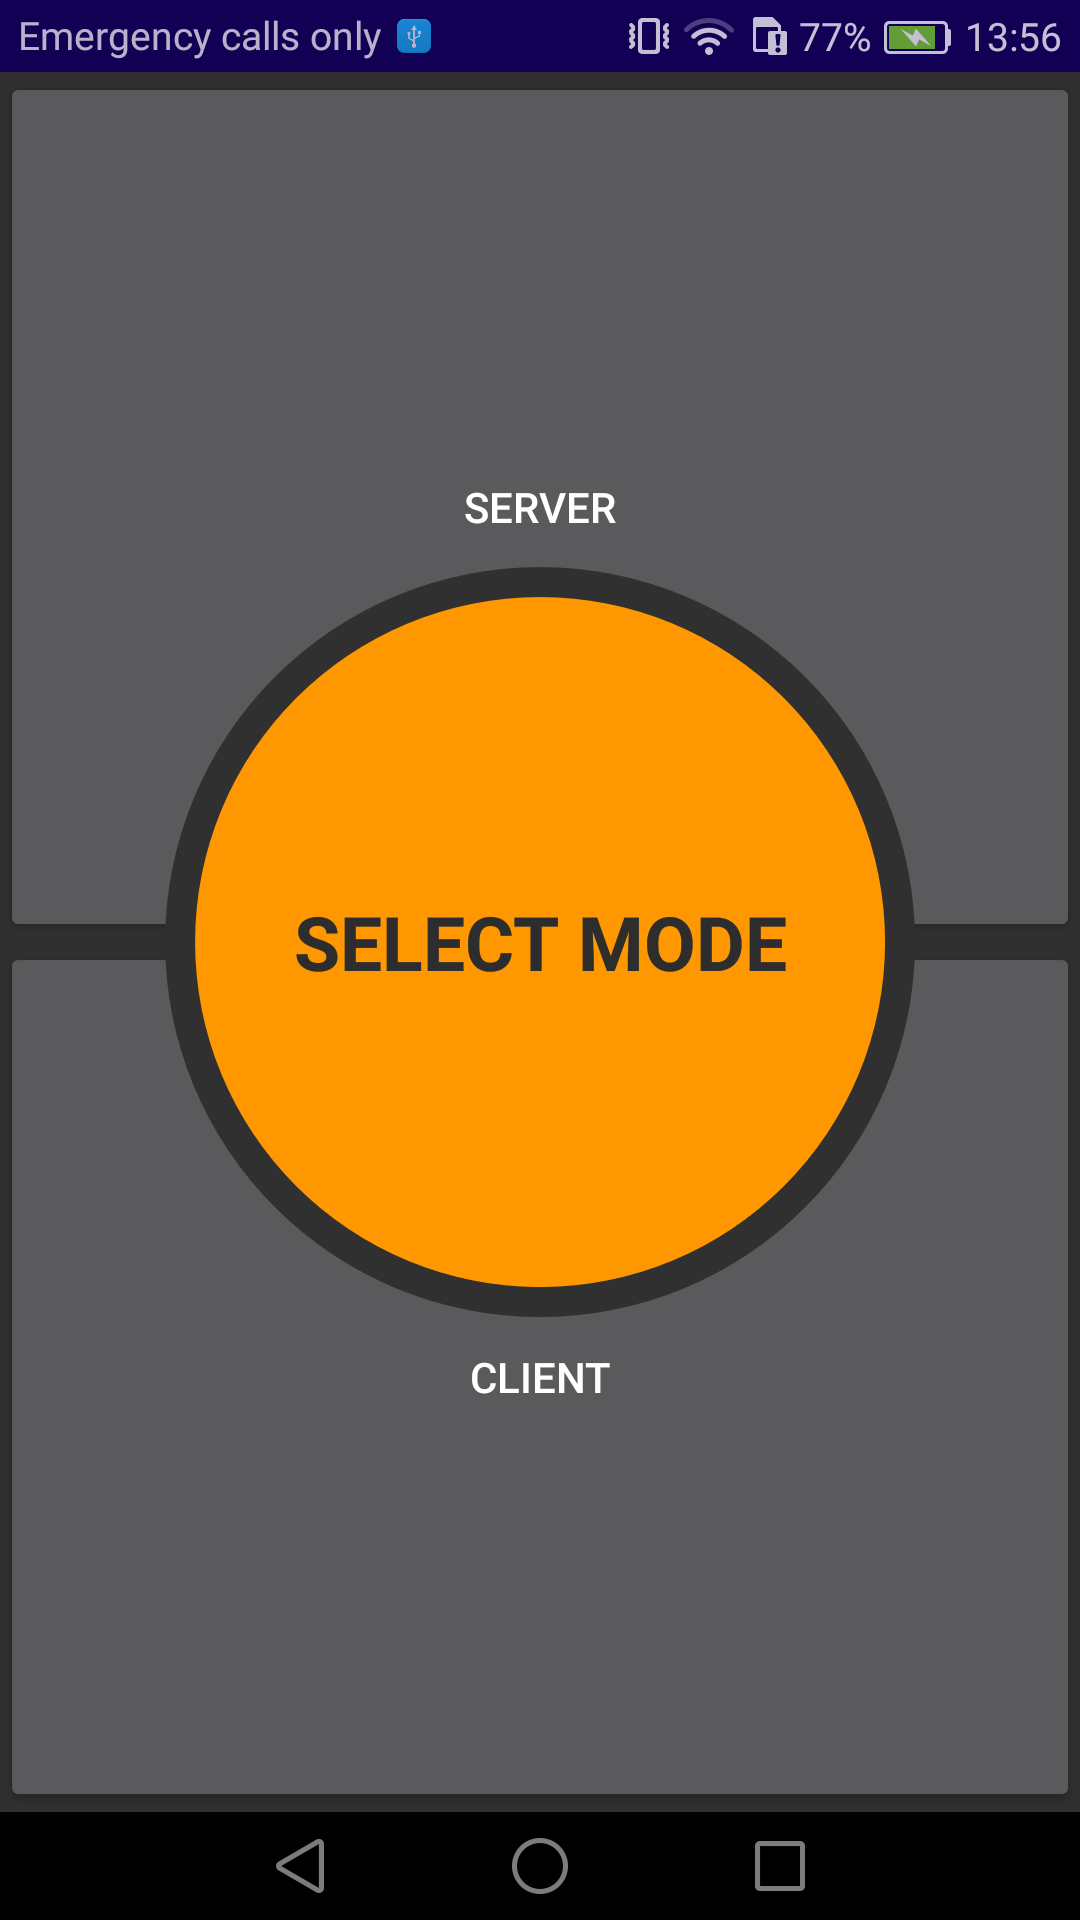
\includegraphics[trim={0cm 0cm 0cm 0cm}, clip, height=7cm]{img/ui/mode_selection.png}
    \caption{Mode Selection}
    \label{fig:mode_selection}
    \vspace{4ex}
  \end{subfigure}%%
  \begin{subfigure}[b]{0.33\linewidth}
    \centering
    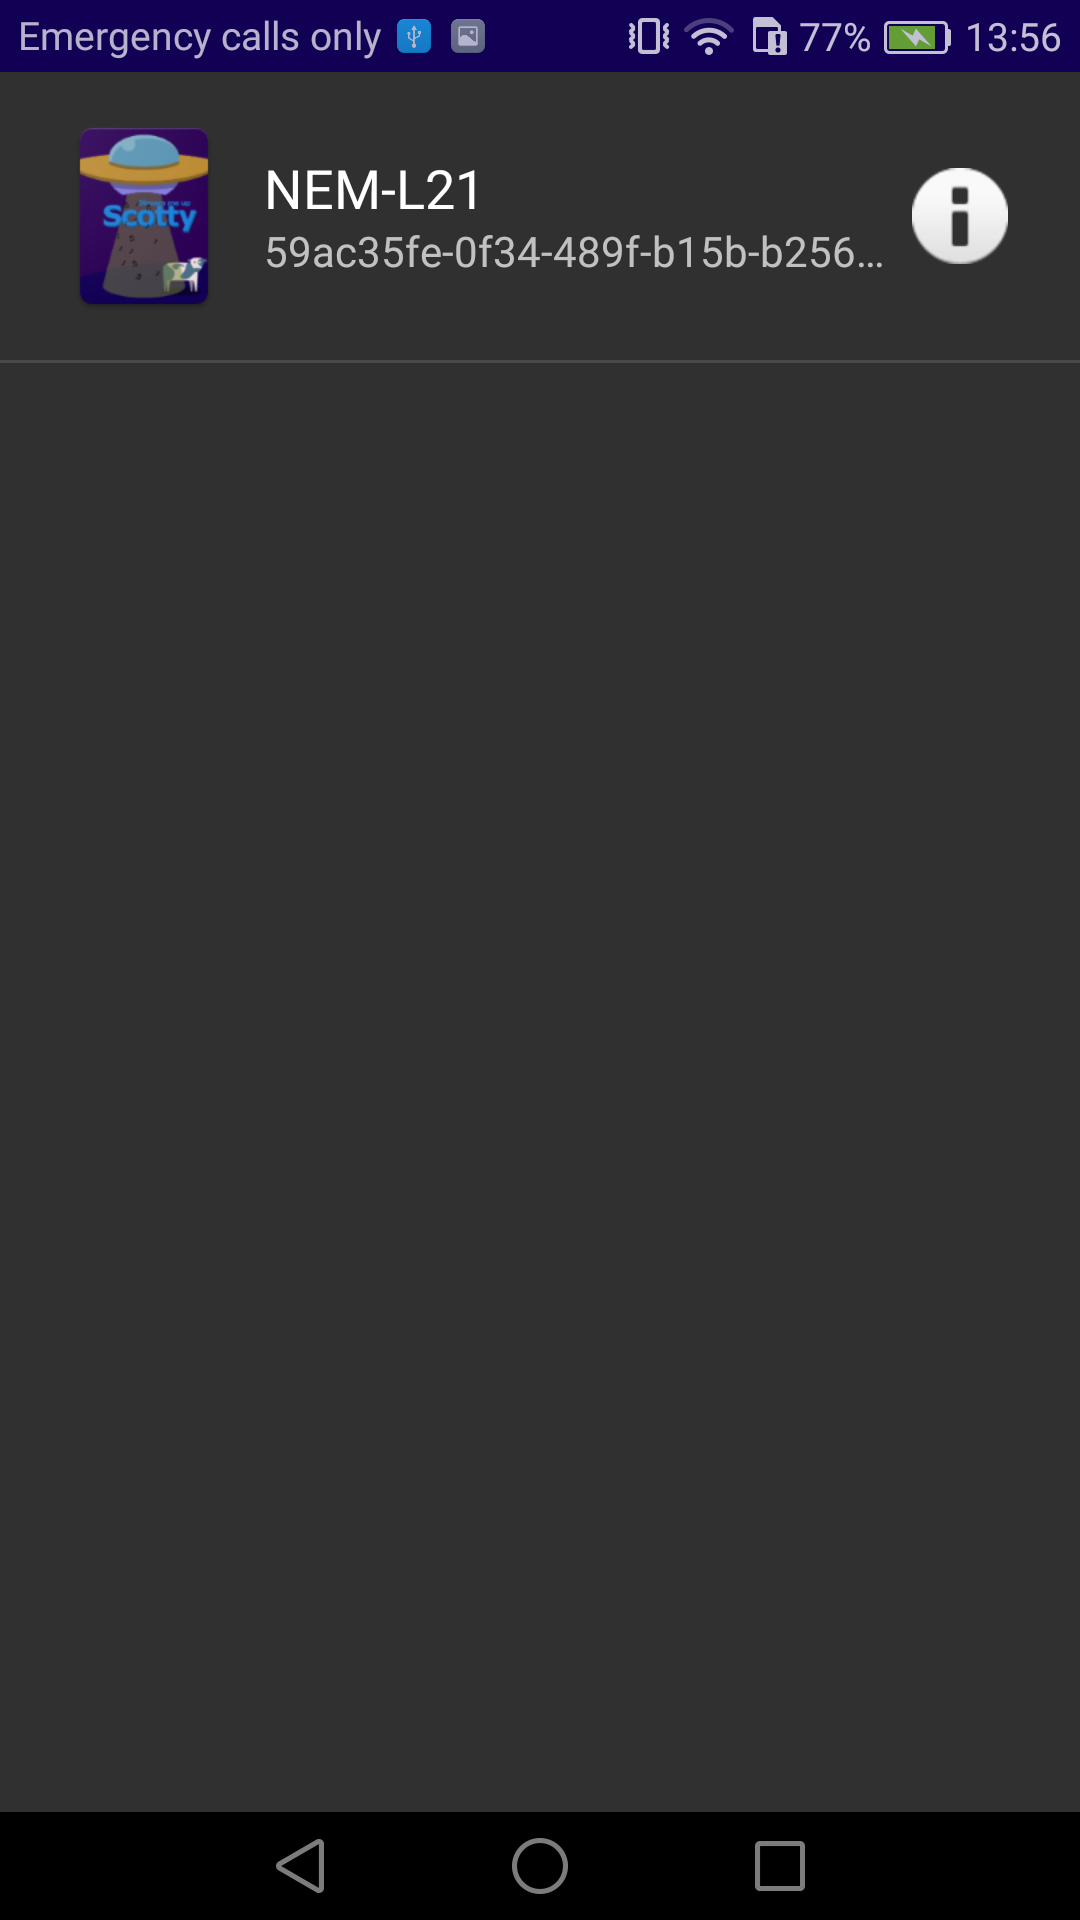
\includegraphics[trim={0cm 0cm 0cm 0cm}, clip, height=7cm]{img/ui/group_selection.png}
    \caption{Group Selection}
    \label{fig:group_selection}
    \vspace{4ex}
  \end{subfigure}%%
  \begin{subfigure}[b]{0.33\linewidth}
    \centering
    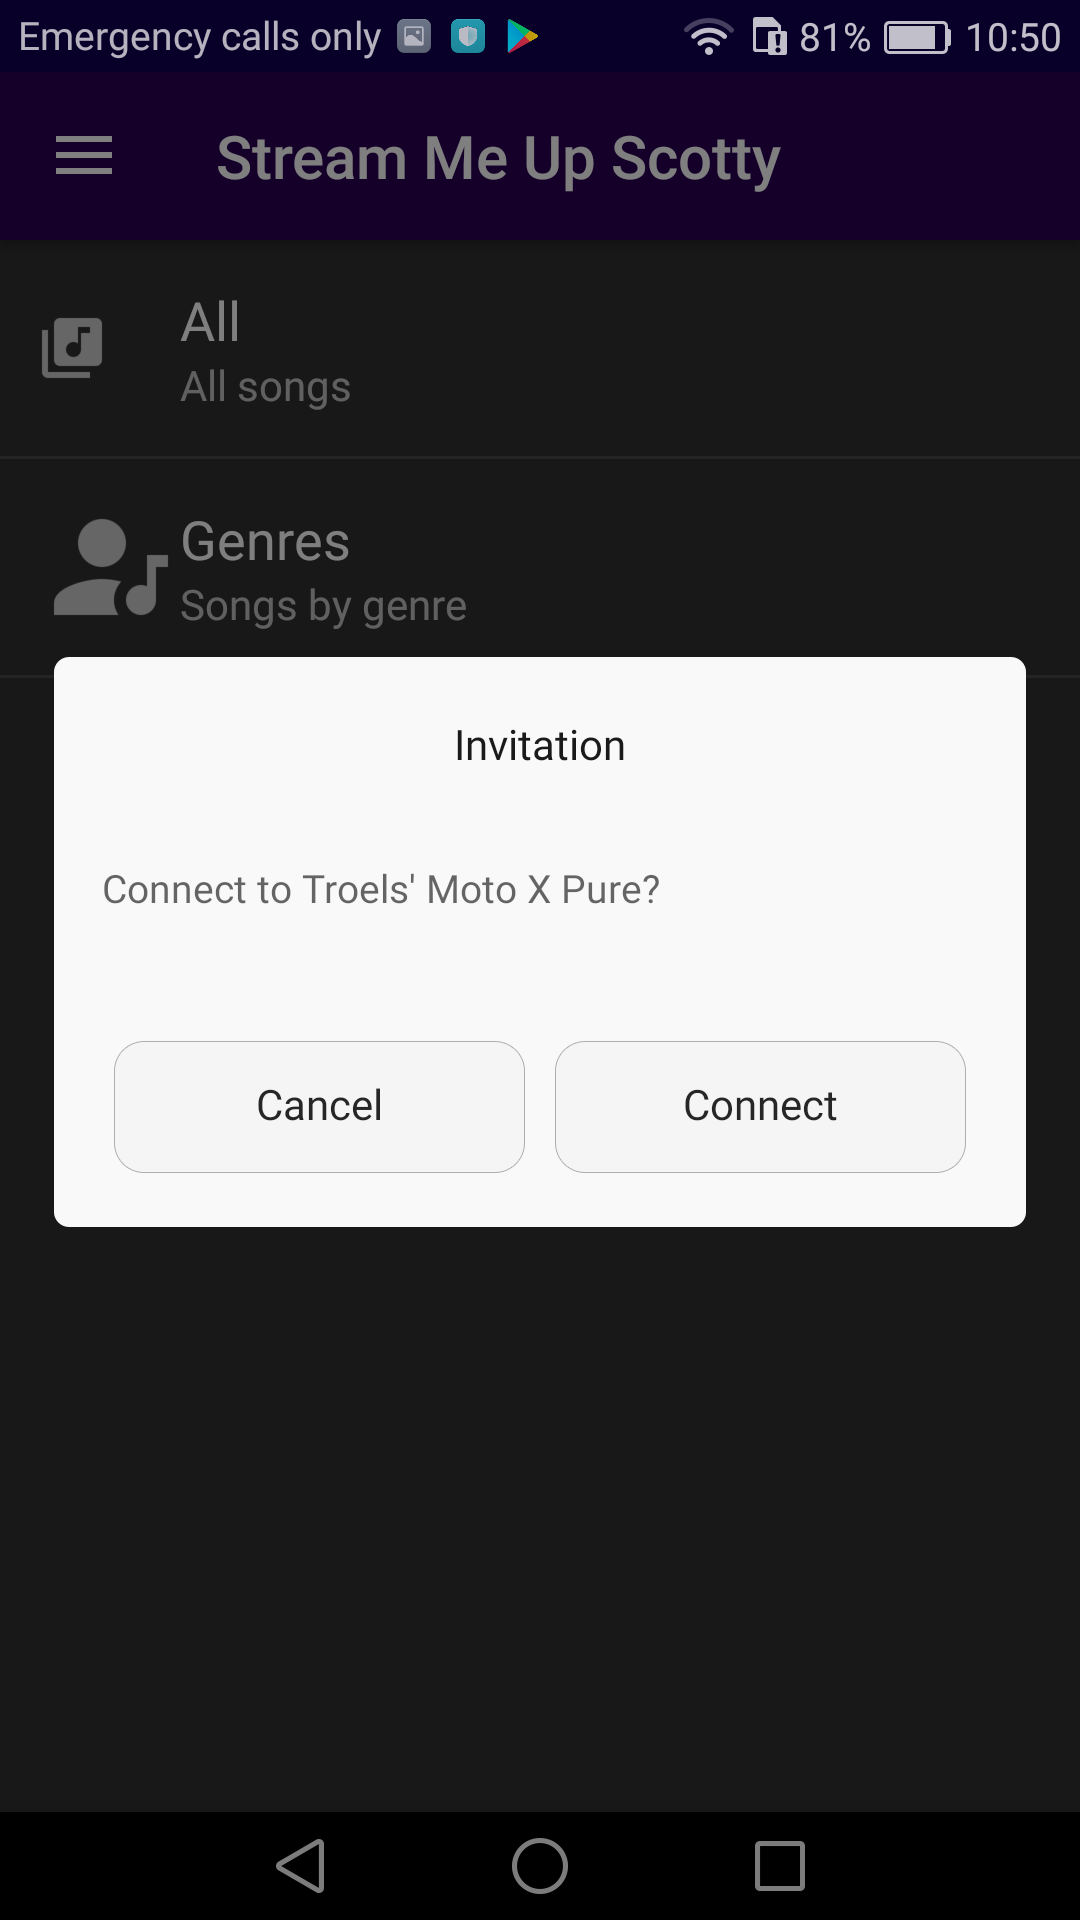
\includegraphics[trim={0cm 0cm 0cm 0cm}, clip, height=7cm]{img/ui/wifi_direct_invitation.png}
    \caption{WiFi Direct invitation}
    \label{fig:wifidirectinv}
    \vspace{4ex}
  \end{subfigure}
  \caption{The user interface relevant for connecting devices.}
  \label{fig:connecting}
\end{figure}

\subsection{Service Discovery}

The first problem which must be handled in order to connect devices is: discovering peers.
Fortunately a part of the WiFi Direct standard is the so called services.
Part of the services is ``Service Discovery'', which is made for the exact purpose of discovering peers.
In Android WiFi Direct is called: ``Wi-Fi peer-to-peer'' or ``Wi-Fi P2P'' for short.\footnote{\url{https://developer.android.com/reference/android/net/wifi/p2p/WifiP2pManager.html}}.

We experienced several issues implementing service discovery in our app, most notable is group negotiation.
When devices connect using WiFi Direct, they negotiate about having the role of group owner.
The group owner is the master of the network, and is responsible for granting new devices access etc.
For our app we want the device which is the server, to also have the role of being the group owner of the WiFi Direct network.
The root of our problem was the fact that the devices would keep a record of the last 32 WiFi Direct groups which the had been a part of, as well as who were the group owner.
This would then become a problem, when one started a new session using the same devices as a previous one, but with a different master.

In order to prevent this issue, we decided to erase the records of previous WiFi Direct networks, when we start discovering services.
In addition to the server creating a new group, once it starts broadcasting its service.
That means that the only preexisting group when a device connects is the one just created by the server.
Since there is a preexisting group, then new devices will try to join it, when connecting.

Connecting to a WiFi Direct network requires approval from the group owner.
The UI shown is dependent on the Android version, and styling by the manufacturer.
An example of it is shown on \cref{fig:wifidirectinv}.

To explain how this occurs we have constructed an slightly simplified UML sequence diagram, on \cref{fig:seq_server_client}.
After the service discovery and the client joining the group, it gets the network info, that is an IP of the group owner.
This is used in the next step, which is establishing a persistent socket.

\begin{figure}[h]
    \resizebox{!}{0.90\textwidth}{
        \begin{sequencediagram}
            \newthread{s}{Server}
            \newinst{sn}{Server Network}
            \newinst[2]{wd}{WiFi Direct}
            \newinst[2]{cn}{Client Network}
            \newthread{c}{Client}

            \begin{messcall}{s}{Start}{sn}{}
                \begin{messcall}{sn}{\shortstack{Announce \& \\\\Create Group}}{wd}{}
                    \begin{messcall}{c}{Start}{cn}{}
                        \begin{call}{cn}{Discover}{wd}{}
                        \end{call}
                        \begin{messcall}{cn}{Services}{c}{}
                        \end{messcall}
                        \begin{call}{c}{Connect}{cn}{Network Info}
                            \begin{call}{cn}{Join Group}{wd}{Network Info}
                                \begin{call}{wd}{Accept?}{sn}{Network Info}
                                    \begin{call}{sn}{Accept?}{s}{ACK}
                                    \end{call}
                                \end{call}
                            \end{call}
                        \end{call}
                        \begin{messcall}{cn}{\shortstack{Establish\\\\Socket Connection}}{wd}{}
                            \begin{messcall}{wd}{\shortstack{Accept\\\\Socket Connection}}{sn}{}
                            \end{messcall}
                        \end{messcall}
                    \end{messcall}
                \end{messcall}
            \end{messcall}
        \end{sequencediagram}
    }
    \caption{Sequence diagram, depicting how our the server announces its service and clients connects.}\label{fig:seq_server_client}
\end{figure}


\subsection{Establishing a Persistent Socket}

After the the client(s) have discovered the server, they will establish a persistent connection.
They are at this point part of the same WiFi Direct network, and the client has just received the IP of the group owner.

When the server first started, it lauches a seperate thread which open a \code{ServerSocket} which accepts incoming socket connections.
After accepting them it creates a MessageConnection which is our abstraction which is run on a seperate thread for each connection from the server to the client, and vice versa.
That thread then continuously tries to read on the socket, to accept messages sent to it.

\subsubsection*{Using Protobufs}
As previously mentioned we decided to use protobufs to serialize our messages.

The protobufs we use can be separated into three groups: Meta-data, commands and data. \tnote{Tids ting går her under meta-data, er det fair?}
\begin{description}
    \item[Meta-data] \hfill \\
        Meta-data is information about the data, the data in this case is the audio data.
        The purpose of sending meta-data is twofold: We send it such that the clients can present it in their UI, and such that our audioplayer can be setup correctly.
        Our meta-data contains the following:
        \begin{itemize}
            \item Artist name
            \item Album name
            \item Song name
            \item Album art url (An optional url containing an image to be displayed)
            \item Song duration
            \item Media-info
        \end{itemize}
        Here the media-info contains the following information about the audio data (in the PCM format). \tnote{Ref til Marcs afsnit om playback med begreberne}
        \begin{itemize}
            \item Sample rate
            \item Channels
            \item Encoding (bit depth pr. channel)
            \item Frame size
        \end{itemize}
    \item[Commands] \hfill \\
        Commands are used to change the playback on other devices.
        All commands contain a timestamp at which the given command should occur. \tnote{Evt. ref til core idea?}
        In total we have the following commands:
        \begin{description}
            \item[PlayCommand]
                Used to start audio playback.
                Contains the location in the audio file to resume playback at, and the timestamp at which the playback should start.
            \item[PauseCommand]
                Used to pause audio playback.
                Much like the PlayCommand, it contains the location in the audio file at which the playback is pause, and the timestamp for when the pause should occur.
            \item[SeekCommand]
                Used to seek in the audio file, i.e. change which part of the audio file should be played.
                As the Play- and PauseCommands, it contains the location which the playback should change to, and the timestamp for when the change should occur.
            \item[SongChangeCommand]
                Used to change the audio file which should be played.
                Contains the meta-data for the file which will be changed to, and the timestamp for when the change should occur.
        \end{description}

    \item[Data] \hfill \\

\end{description}